\documentclass{aa}
                                                                            
\usepackage{latexsym}
\usepackage{graphicx}
\usepackage{natbib}
%\usepackage[latin1]{inputenc}
\usepackage{color}

\newcommand{\hs}{\bfseries}
\newcommand{\he}{\rm}
\newcommand{\sect}[1]{Sect.\,\ref{#1}}
\newcommand{\fig}[1]{Fig.\,\ref{#1}}
\newcommand{\tab}[1]{Table\,\ref{#1}}


%\definecolor{dgreen}{rgb}{0,0.5,0}
\newcommand{\nnG}[1]{{{\color{red}{#1}}}}




%-----------------------------------------------------------------------------
\newcommand{\tobedone}[1]{\typeout{----> Warning: something to be done: #1}%
                          {\color{blue}$\to$} \marginparwidth1.1mm 
				\marginpar{\rule[-2mm]{1mm}{6mm}}
                                {{\color{blue}\footnotesize\sf #1}}}
%-----------------------------------------------------------------------------


\sloppy

\begin{document}

%\title{Evolution of passive tracer particles in a 3D rMHD model of the solar corona}
\title{Dynamics of transition region loops in an enhanced network simulation of the solar atmosphere}
%\title{Comparison of low-lying and high-reaching loops in an enhanced network simulation of the solar atmosphere}
\titlerunning{Dynamics of transition region loops}



\author{P. Zacharias \inst{1,2} \and V.H. Hansteen \inst{1,2} \and J. Leenaarts \inst{3}}%\and M. Carlsson\inst{1} \and B.V. Gudiksen\inst{1}}
\institute{Institute of Theoretical Astrophysics, University of Oslo, P.O.Box 1029 Blindern, 0315 Oslo, Norway \and Rosseland Centre for Solar Physics, University of Oslo, P.O. Box 1029 Blindern, NO-0315 Oslo, Norway \and Institute for Solar Physics, Department of Astronomy, Stockholm University, AlbaNova University Centre,
106 91 Stockholm, Sweden}

%--------------
\abstract%
%
{%---CONTEXT---(optional)-----------------------------------------
%
The solar chromosphere and transition region are highly dynamic and therefore hard to study. 
%Different kinds of processes, such as waves, electric currents and magnetic reconnection events are known to contribute to the heating of the outer solar atmosphere, but it still not well understood how much each process contributes and how it depends on the local plasma conditions. 
State-of-the art numerical models have now become sufficiently advanced to allow detailed studies of transient events on various scales in space and time. 
%a detailed comparison with high-resolution high-cadence observations on small scales. Only recently, this combined approach has led to the discovery of the unresolved fine structure (UFS) loops. 

%These recent advancements, in combination with a new analysis tool for the 3D numerical experiments for the first time, allows to 
%their underlying magnetic structure is changing on small timescales. Therefore, this region of the solar atmosphere has been notoriously hard to study.  
%highly dynamic and complex magnetic structure of the solar atmosphere ...
%Following magnetic field line in time thoroughly in 3D MHD models of the solar atmosphere has always been challenging. One is limited by .... and relies on methods and assumptions that are simply taken as granted, because there is no better way to do it. 
%The highly complex structure and magnetic coupling, riddled by waves of different kinds, ... , makes it hard to believe that this is accurate enough. 
%This highly dynamic interface region has been notoriously hard to study.

%We use one of the most advanced 3D rMHD codes, the Bifrost code for our simulations as well as a typical magnetic field setup.

%The method we apply is very comparatively simple. We implement tracer particles into the simulations, referred to as corks, that are passively advected by the plasma flows. 
%In order to support a million degree corona ..., a continuous mass supply of the order of ...  appears to be necessary.  However, this undertaking might give some far-reaching answers to these questions can shed light on important questions such as the heating of the outer layers of the solar atmosphere and the damit verbundenen ... processes which contribute energy ....  highly dynamic and shows transient events on various scales in space and time. Most of these features are related to changes in the magnetic field structure or impulsive heating caused by the conversion of magnetic to thermal energy.
%
}{%---AIMS---------------------------------------------------------
%
The dynamics of cool, low-lying transition region loops and hot, coronal loops are compared. 
%, in order to obtain insights on their role in the chromosphere-corona mass cycle.
Based on the evolution over several minutes, we are able to characterize various kinds of waves that are travelling along the loops. 
%and investigate the processes that lead to the exchange of mass between the different atmospheric layers. By quantifying physical parameters such as mass, velocity, and orientation of the plasma ejection relative to the magnetic field, 
 %thus aiming at a more complete picture of what is actually happening during the simulation. 
}{%---METHODS------------------------------------------------------
%
Passive tracer particles (so-called corks) are implemented into a three-dimensional numerical experiment of the solar atmosphere and advected by the plasma flow, while the code is running. By following the cork trajectories, we have a new, highly accurate tool to follow magnetic field lines over time in the simulations. %Here, this approach is applied to the study of magnetic structures of various size and temperature. 
}{%---RESULTS-----------------------------------------------------
%
%The importance of the cork-based approach in order to follow magnetic field lines in time is highlighted by a comparison with the VAPOR field line advection algorithm. 
We compare the evolution of different sets of low-lying and high-reaching loops and present examples of each type. Typical lifetimes of 10-15~min are found for transition region loops, whereas the lifetimes of coronal loops in the model exceed the duration of the simulation span that has been analyzed (25~min). Space-time maps of various plasma parameters give insight on the evolution of the loops in connection with the heating and cooling processes of the plasma. In addition, the decomposition of the velocity vector into components parallel and perpendicular to the magnetic field elucidates the various kind of waves propagating along the magnetic field lines. Magnetoacoustic waves with a frequency of $\sim 0.005 $~s$^{-1}$ are omnipresent {\color{blue}leading to} the swaying of the field lines and their periodic variation in height. Torsional Alfv\'en waves in the model are often associated with jets of cool plasma that can reach up to 10~Mm in height and last for approximately 10~min. The acceleration force of these cool plasma jets is the combined action of the Lorentz force and the buouyancy force. 
%..  rapidly changing nature of transition region loops. 
%
}{%--CONCLUSIONS---(optional)-------------------------------------
%
Our findings imply that a highly accurate scheme is necessary in order to follow magnetic field lines in time and identify wave-like motions. With a cork-based approach, we are able to identify magneto-acoustic waves as well as Alfv\'enic waves that are travelling along the magnetic field lines.  
%
}%--------------------------------------------------------------
%
\keywords{     Stars: coronae
           --- Sun: corona
           --- Sun: transition region
           --- Sun: UV radiation
           --- Techniques: spectroscopic}
%---------------------------------------------------------------


\maketitle







\section{Introduction}
Coronal loops are considered to be the basic building blocks of the solar corona. Due to the high conductivity and as the magnetic energy dominates over the thermal energy in this region of the Sun's atmosphere, the plasma is confined to field lines channeling the plasma flows. The energy is rapidly distributed along those field lines due to the efficient heat conduction, resulting in loop-like structures aligned with the magnetic field. %At chromospheric heights, the magnetic field outside sunspots is concentrated in a network defined by the super-granulation. 
In the 1970s, it was suggested that magnetic structures rapidly expand into the corona in the form of so-called coronal funnels, which dominate the low corona \citep{gabriel:1976}. 
As a result of measurements with improved spectral and spatial resolution, it became apparent that the original, simplified picture of the solar atmosphere needed to be modified. Indirect spectroscopic evidence from the High Resolution Telescope Spectrograph (HRTS) and Skylab spectra led to the introduction of the term unresolved fine structure (UFS) by \cite{feldman:1983} and the hypothesis that the plasma in the solar transition region appears in structures magnetically isolated from the chromosphere and corona. The existence of a multitude of loops of different sizes and temperatures below and between the coronal funnels was suggested by \cite{dowdy:1986}, in order to reproduce the correct shape of the emission measure (EM) below 100\,000~K. Static, low lying loops were shown to account for the rise of the differential emission measure (DEM) at low temperatures by \cite{antiochos+noci:1986}, however, \cite{cally+rob:1991} found that such cool loops are thermally unstable. Using transient one-dimensional heating models to investigate the hydrodynamic behavior of small cool magnetic loops, \cite{spadaro+al:2006} were able to show that small cool structures can produce the observed emission measure distribution and over the entire temperature range, as well as the temperature dependence of the persistent redshifts, provided the heating is spatially localized near the chromospheric footpoints. The high spatial and temporal resolution observations obtained by the Interface Region Imaging Spectrograph (IRIS) have finally revealed observational evidence for the existence of the UFS \citep{hansteen+al:2014}. These structures are shown to be short, bright and low-lying varying rapidly on the time scale of minutes. Nowadays, extensive radiative-MHD simulations \citep{gudiksen+al:2011} enable full forward-modelling of the solar atmosphere from the convection zone to the corona at a spatial and temporal resolution suitable for comparison with observations \citep{carlsson+al:2016}. Comparisons with such numerical models showed that low-lying episodically heated loops naturally arise in the state-of-the-art 3D MHD models \citep{gudiksen+al:2011,carlsson+al:2016}, which can thus be used as guidance to exploit their properties in greater detail.\\ 



%When investigating the relationship between plasma structures and magnetic field lines, one usually depends on two related assumptions, {\emph{i.e.,}} the plasma structures trace magnetic field lines at any given instant in time and the structures trace the same field line during their life time. On the other hand,
The evolution of the magnetic field lines themselves is rather complex, and the field lines, in general, cannot be thought of as a static background \citep[see, {\emph{e.g.}},][]{leenaarts+al:2015}. 
%Thus, in order to follow the magnetic field lines in time, further approximations are required or novel techniques need to be applied. 
In this study, we present results obtained based on a novel technique of following magnetic field lines over time, which is based on the implementation of passive tracer particles in the Bifrost stellar atmosphere code \citep{zacharias+al:2018}. Whereas earlier approaches have often been limited by the finite time resolution of the snapshot series (typically 10~s cadence), this new approach allows us to follow test particles at highest cadence possible (i.e., timestep cadence of the code) and thus to determine the evolution of the field lines most accurately. We present results from a comparison between low-lying transition region loops and high-reaching coronal loops in a three-dimensional magnetohydrodynamic (3D MHD) experiment of the solar atmosphere above an enhanced network region. The formation and propagation of a cool chromospheric plasma jet, which appears above a strong magnetic field concentration, is found to be associated with the passage of a torsional Alfv\'en wave, the properties of which are analyzed.\\
%{\color{red}For cool brightenings moving upwards, see Introduction of blob paper...}\\



%We take this approach one step further, and investigate the temporal evolution of magnetic field lines more accurately by implementing passive tracer particles into the Bifrost stellar atmosphere code. The corks are advected by the plasma flow while the code is running, thus their trajectories offer the most precise way to follow structures over time in the simulation. The corks also allow to investigate fast mode MHD waves, which are present in the Bifrost models, but cannot be easily identified in the field-line-based approach \citep{leenaarts+al:2015}. 

This work is organized as follows. In section \ref{sim_section}, the simulations are introduced. Section \ref{analysis_section} outlines the new cork method and describes the tracing of the  magnetic field lines in time. In section \ref{results_section}, the results of our field line analysis are presented. 
%Section \ref{} goes beyond this approach and focuses on the corks' more general behaviour. 
%We conclude this study with a discussion (section 5) and outlook section (section 6).
We conclude this study with a discussion, which puts this work in context with other studies (section \ref{discussion}).

%During the last decade, rapid advances in computing capability have revolutionized the state-of-the art numerical simulations and their capabilities in interpreting observations. Nowadays, extensive radiative-MHD numerical simulations enable full forward-modelling of the solar atmosphere, from the convection zone to the corona (Gudiksen et al. 2011). Advances in algorithms, supercomputing capability, and parallelization techniques allow computations at a spatial and temporal resolution that is suitable for comparison with observations (Carlsson et al. 2016). 
 
%The old standard picture of the magnetic structure of the solar transition region (Gabriel et al. 1976)
%The discovery of UFS: Introduction of the term unresolved fine structure (UFS) in 1983 by Feldman (): solar plasma in the transition region appears in structures magnetically isolated from the chromosphere and corona. 
%Two-component transition region: Dowdy

%State of the art observations and simulations: 
%Multi-component transition region: Peter 2000
%Transient heating models: Spadaro et al. 2006
%UFS in IRIS observations
%UFS in 3D MHD models of the solar atmosphere 
 

%Why and how do the loops form, what sets their height?



%{\color{red} A caveat to this discussion is that the
%magnetic field needed to describe the upper atmosphere is observationally not well constrained
%and that a number of highly dynamic events such as spicules of type II are not
%reproduced.\\

%The compressive modes (acoustic waves and
%slow mode waves in the low-? upper chromosphere) rapidly become non-linear with
%height and dominate the dynamics and energetics of large parts of the chromosphere.
%At greater heights these waves are channeled by the magnetic field. The magnetic
%field, when strong, is also a direct source of heating, as currents dissipate through Joule
%heating in regions of large magnetic gradients. Thus, we find higher chromospheric
%temperatures near regions of enhanced magnetic field strength.}

%The outer solar atmosphere is highly structured and very dynamic. This ranges from large disruptive events such as flares and coronal mass ejections (CMEs) down to small-scale explosive events in the transition region between the chromosphere and the corona. Because the coronal dynamics are a direct signature of the processes governing the energy balance in the upper atmosphere, i.e., coronal heating, radiative losses and heat conduction, the investigation of coronal transients on all temporal and spatial scales is a key for also understanding the nature of the corona of the Sun and other stars. We present results from a three-dimensional magnetohydrodynamic (3D MHD) numerical experiment of the solar corona in which an explosion-like event drives a confined plasma ejection ballistically through the corona along the magnetic field lines. 

%Reference to Mats' 2015 paper IRIS/Bifrost...\\
%In a recent study, Golding et al. 2015 showed the importance of non-equilbrium helium ionization for the dynamics and thermal structure of the upper chromosphere and transition region. It might also help resolve the problem that intensities of chromospheric lines computed from current models are smaller than those observed.


\section{Setup of the numerical experiment}\label{sim_section}
%We analyze the structure and dynamics of several transition region loops and a cool plasma jet in a 3D MHD simulation of the solar atmosphere above the enhanced network. 

%At the core of the code is a staggered mesh explicit code that solves the standard MHD partial differential equations (PDEs) on a Cartesian grid:

The setup of the 3D model is identical to the one described in \cite{zacharias+al:2018}. The simulations have been performed with the Bifrost stellar atmosphere code \citep{gudiksen+al:2011}, a staggered mesh explicit code that solves the standard MHD partial differential equations on a Cartesian grid, which extends from the upper convection zone to the low corona. The box size is 24x24 Mm$^2$ in horizontal direction and $\approx$17 Mm in the vertical; it reaches -2.4 Mm below the solar surface and 14.4 Mm above. The simulation has a size of 504x504x496 grid points corresponding to a resolution of $\approx$48~km in the horizontal direction. In the vertical direction, a non-equidistant grid spacing is applied, and the resolution ranges between $\approx$19 km in the photosphere and transition region to $\approx$100 km in the corona, where the temperature and density gradients are less pronounced. 
%The magnetic field configuration is a so-called enhanced network simulation consisting of two magnetic field concentrations separated by approximately 8 Mm. For more details, we refer the reader to \cite{gudiksen+al:2011}.

The magnetic field configuration is chosen in a way that it leads to a small network-like configuration. It was created by specifying the magnetic field at the bottom boundary and using a potential field extrapolation to compute the field in the entire computational domain. The magnetic field was inserted into a relaxed hydrodynamical simulation and was then allowed to evolve freely. The simulation was run for 3000~s of solar time using LTE ionization, before non-equilibrium hydrogen ionization was switched on for 830~s. Afterwards, starting from $t$=3850~s, the simulation was run for 1500~s of solar time without non-equilibrium hydrogen ionization including passive tracer particles. For more details, the reader is referred to Carlsson et al. (2016).
%Bifrost is an explicit code with diffusive terms in the equations in order to ensure stability and to ensure that structures smaller than the grid size cannot develop. The diffusive operator employed is split in a small global diffusive term and a location specific hyper diffusion term (see Eq. (9) in Gudiksen et al. 2011). Spatial derivatives and the interpolation of variables are done using high order polynomials. The equations are stepped forward in time using the explicit third order predictor-corrector procedure described by Hyman (1979).

%The simulations are set up in a way to study processes in the solar chromosphere and transition region with a magnetic field configuration characterized as ?enhanced network?. 
The magnetic field at the bottom boundary consists of two patches of opposite polarity separated by 8 Mm with an overall balanced flux.
The average unsigned magnetic field strength in the photosphere is 48 G (5 mT). The magnetic field distribution does not change significantly during the simulation timespan.
Both the top and the bottom boundaries are transparent. At the bottom boundary, the magnetic field is passively advected with no extra field fed into the computational domain. The effective temperature of the simulated atmosphere is not set directly, but only indirectly by specifying the incoming entropy flux at the lower boundary. The average temperature in this model is maintained by fluid motions in the convection zone, by radiative transfer in the photosphere, by the balance between acoustic shocks and radiative losses in the lower chromosphere, and by the balance of Joule and viscous heating, thermal conduction, and radiative losses in the upper chromosphere, transition region and corona. 

%
%The code is massively parallelised and the simulations were carried out on vilje (NOTUR). They were run for approximately ... on ... cpus. For the purpose of this study, neither hydrogen nor helium non-equilibrium ionization is considered, which considerable reduces the computational time needed.  
%
%
%\begin{figure*}[!h]
%\begin{center}
%\includegraphics[width=0.3\textwidth]{figures/bz_atz416_385.eps}
%\includegraphics[width=0.3\textwidth]{figures/temperature_histo_385_nolog.eps}
%\includegraphics[width=0.3\textwidth]{figures/density_histo_385.eps}
%\end{center}
%\caption{{\it{Left panel}}: Initial vertical magnetic field at $z$=0 Mm, i.e., photospheric height. {\it{Middle and right panel:}} Initial temperature and density distribution as a function of height in the form of a 2D histogram. The gray lines indicate the average value of temperature/density at each height. \label{bz_atz416_385}}
%\end{figure*}
%

%In addition, 



%, which corresponds to a total of 125991936 individual corks that are followed over time. The snapshot cadence for writing out the basic MHD parameters during the simulation is 10 seconds, and we chose the same cadence for writing out the cork positions. This doubles the amount of output data, however, little extra time is needed for the calculation and writing of the additional corks data.

%\section{Method and Analysis}
%
%\subsection{Corks}
%The large number of corks that were traced during the simulation (125 million) allows us to perform both statistical studies of the different physical parameters, including temperature, density and velocity, as well as their collective cork behavior. This is done in Paper 1 of this series. In this study, we focus more on studies of individual cork tracks... In a follow up paper, we will look at the energetics of different explosive events...
%In the setup we use, the corks are unique and labeled according to their initial grid position. This allows us to also follow them individually and to analyze their tracks.\\
%Tracing / How accurate\\
%Resetting, comparison\\
%Corks that end up on top/bottom of the box... How many?\\
%Cubic spline (?) interpolation to extract physical parameters.\\
%Mention waves in the chromosphere ...\\
%Mention field line analysis. Is this something we treat in this paper?
%


\section{Analysis method}\label{analysis_section}\label{section_VAPOR}
Passive tracer particles, so-called corks, have been implemented into the Bifrost simulations \citep{zacharias+al:2018}. Initially, corks are placed at every point of the simulation grid; we then follow them in time for approximately 25 min. For the tracking of each cork in the simulation, the plasma flow at the respective cork position is considered for every single timestep. The position ${\vec{r}}_i$ of a cork labeled $i$ evolves as $\frac{\partial {\vec{r}}_i}{\partial t}= \vec{v}(\vec{r}_i)$, where $\vec{v}(\vec{r}_i)$ is the plasma velocity at the location of the cork. 
The 3D rMHD simulations thus provide us with a vast number of cork trajectories and a unique tool to trace features, such as individual magnetic field lines, over time. 

Fig. \ref{swaying_fieldline} shows projections of a magnetic field line on the $xz$-, $yz$-, and $xy$-planes. The field line has been obtained by tracing the magnetic field vector from the cork position, which is indicated by an asterix. By following the cork trajectory over time, the evolution of the field line is obtained. The corresponding movie (see online material), which shows a swaying motion of a coronal field line, will be discussed in more detail in section \ref{section_coronal_loops}. \\

\begin{figure*}[!h]
\begin{center}
\includegraphics[width=\textwidth]{figures2/xz_yz_xy_line61_385.eps}
\end{center}
\caption{Example of swaying field line. A movie showing the temporal evolution of the field line is found in the appendix. \label{swaying_fieldline}}
\end{figure*}

%{\color{blue} Move section 4.1 here. Done.}\\
%Figures \ref{fig_stmaps_highloops}, \ref{fig_stmaps_lowloops_488}, \ref{fig_stmaps_lowloops_005} and \ref{fig_stmaps_wave} show 
The time evolution of various plasma parameters along a field line of length $s$ can be represented by space-time diagrams (see, {\emph{e.g.}}, Fig. \ref{fig_stmaps_highloops}). %, which we have selected in order to highlight differences between various kinds of loops present in the enhanced network simulation.  %The seed points of these field lines ... .
The $st$-panels show the evolution of plasma temperature $T$ and density $\rho$ in the first row; plasma-$\beta$, field line curvature $\kappa$ and torsion $\tau$ in the second row; plasma flow speed parallel to the field line $u_{\parallel}$={\bf{u}} $\cdot$ {\bf{b}} and the two transverse directions $u_P$={\bf{u}} $\cdot$ {\bf{P}} and $u_N$={\bf{u}} $\cdot$ {\bf{N}} in the third row. This representation makes it easy to distinguish between disturbances propagating along or perpendicular to the magnetic field. In the fourth row, we show the divergence of the plasma flow parallel to the magnetic field ($\nabla_{\parallel} \cdot {\bf{u}}=\partial u_{\parallel}/\partial s$), the divergence of the flow field perpendicular to the field ($\nabla_{\perp} \cdot {\bf{u}} = \nabla \cdot {\bf{u}} - \partial u_{\parallel}/\partial s$) and the vorticity parallel to the magnetic field. The fifth row shows the evolution of the adiabatic heating rate ($Q_{\rm{pdV}}$), the Joule heating rate ($Q_{\rm{Joule}}$), and the viscous heating rate ($Q_{{\rm{visc}}}$) per particle along the field line.\\ 


%{\color{blue}Move to previous section! Done.}
In the following, we are focusing on a time sequence of about 25 minutes duration in the numerical experiment. All points of time discussed here refer to time $t$=0 at the beginning of this sequence. This is the time, when the corks are implemented into the simulation. The actual simulation was started long before $t$=0, so that any impact of the initial condition is excluded during the investigated time sequence.






%Note that the original Bifrost format is with the z-axis going downwards. In order to obtain a right-handed coordinate system, the (x,y) coordinate system has been mirror imaged compared with a normal definition (see IRIS technical note 33). Some earlier papers (e.g., Zacharias et al. 2017a, Leenaarts et al. 2015) show data mirror imaged compared with the published data. It is only when dealing with vector quantities (e.g., magnetic field) that this makes a difference. 

%The field-line based analysis approach only brings forward waves that travel parallel to the magnetic field. The third classical MHD waves, the fast mode, can propagate at an angle to the magnetic field.

%The loops connecting the two dominant magnetic field concentrations are rather hot loops as can be seen from Fig. \ref{}. 
%We have many VAPOR plots and movies showing the emission of si4, o6 and ne8 together with those field lines. 
%{\color{red}Anhand einzelner Beispiele zeigen wir im Folgenden welche Art von Wellen sich in der Simulation ausbreiten.}
%In the following, we continue the discussion started in ... and extend the analysis beyond corks at $T$=100\,000~K. 

%\begin{itemize}
%\item loops\_1k: 2600 field lines between 3850 and 5300s. Corks have z=1 Mm at t=3850s
%\item lines\_upper\_tr
%\item lines\_low\_tr
%\item lines\_red\_right\_low2
%\item iso/tracks: (2725,7)
%\item iso/TR\_tracks: (27246,7): 27246 lines between 4970 and 5030s. Corks have logT=[4.99,5.01] at t=5000s. 
%\item lowloops: zz=200 (z=4.3 Mm): stmaps on braeburn only: data/cb24bi\_corks\_norelocate\_more/plots/lowloops/stmaps/: 512 out of 625 lines
%\item highloops: zz=78 (z=8 Mm): stmaps on braeburn only: data/cb24bi\_corks\_norelocate\_more/plots/highloops/stmaps/: 512 out of 625 lines
%\end{itemize}

%Presence of compressible longitudinal slow-mode waves, which steepen to shocks at chromospheric heights and propagate with speeds close to the sound speed. 

%{\color{red} Do we see any wave-patterns in the cork columns here, i.e., in highloops, lowloops, lowloops2.}

%Nearly incompressible transverse waves that propagate with Alfv\'enspeed. 




\section{Results}\label{results_section}

We start this section with a discussion on the importance of using corks for the field line tracing (section \ref{section_vapor}).
%We start this section with a description of the various plasma parameters that are investigated in the following (section \ref{description}).
We then focus on two different sets of magnetic field lines, namely coronal field lines (section \ref{section_coronal_loops}) and transition region field lines (section \ref{section_TR_loops}), and investigate their properties and their temporal evolution during the simulation. In particular, we analyze the various kinds of waves that are found to propagate along these loops. 
In section \ref{section_cool_plasma}, we study the evolution of a field line bundle, which is associated with a cool plasma ejection {\color{blue} and an Alfv{\'e}nic wave}.
%In section \ref{section_TR_loops2}, we return to the set of field lines, which was the matter of discussion in Zacharias et al. 2017a. Here, we investigate the long-term evolution of the transition region loops rather than the one-minute evolution of corks at $T$=100\,000~K. 

%a closer look at the structure of the atmosphere above the enhanced network, as well as a comparison between our new field line based approach and other methods based on {\emph{e.g.}, field line advection. 
%two more sets of field lines, which are identified with ... a couple of interesting examples by extracting field lines from a field line bundle, and  ...}

%\begin{itemize}
%\item Is there a difference in height of the TR between transition region and coronal loops?
%\item waves reflection, e.g., in the TR?
%\end{itemize}
%all numbers from cb24bi_analyze_random.pro 

%\subsection{Analysis of the Dynamics of Single Field Lines}\label{description}
%Figures \ref{fig_stmaps_highloops}, \ref{fig_stmaps_lowloops_488}, \ref{fig_stmaps_lowloops_005} and \ref{fig_stmaps_wave} show the time evolution of various plasma parameters along the length $s$ of the field line for four different examples in the form of space-time ($st$)-diagrams. %, which we have selected in order to highlight differences between various kinds of loops present in the enhanced network simulation.  %The seed points of these field lines ... .
%The $st$-panels show the evolution of plasma temperature $T$ and density $\rho$ in the first row; plasma-$\beta$, field line curvature $\kappa$ and torsion $\tau$ in the second row; plasma flow speed parallel to the field line $u_{\parallel}$={\bf{u}} $\cdot$ {\bf{b}} and the two transverse directions $u_P$={\bf{u}} $\cdot$ {\bf{P}} and $u_N$={\bf{u}} $\cdot$ {\bf{N}} in the third row. This representation makes it easy to distinguish between disturbances propagating along or perpendicular to the magnetic field. In the fourth row, we show the divergence of the plasma flow parallel to the magnetic field ($\nabla_{\parallel} \cdot {\bf{u}}=\partial u_{\parallel}/\partial s$), the divergence of the flow field perpendicular to the field ($\nabla_{\perp} \cdot {\bf{u}} = \nabla \cdot {\bf{u}} - \partial u_{\parallel}/\partial s$) and the vorticity parallel to the magnetic field. The fifth row shows the evolution of the adiabatic heating rate ($Q_{\rm{pdV}}$), the Joule heating rate ($Q_{\rm{Joule}}$), and the viscous heating rate ($Q_{{\rm{visc}}}$) per particle along the field line. 

\subsection{Field line advection algorithms}\label{section_vapor}

The importance of an accurate field line tracing algorithm becomes clear when comparing the two approaches described below. 
%{\color{blue} This should be a separate section in the Results section! Done}
Field line advection algorithms, such as the one provided by the Visualization and Analysis Platform for Ocean, Atmosphere, and Solar Researchers \citep[VAPOR,][]{clyne:2005, clyne:2007} typically suffer from the ambiguous behaviour of the plasma flow between consecutive snapshots of a time-series. %a short-coming regarding

%{\color{blue}Note: We should save some of this for the discussion. Something like: No information is provided on what is happening to the plasma during the 10 sec timespan.} 

VAPOR supports the option to follow magnetic field lines under the influence of a velocity field, however, it can only do so at timestep cadence (typically 10~sec). The implemented field line advection algorithm is representative for methods that are typically used to follow magnetic field lines in simulations. It is based on the following steps: 
%and it can be used to compare different tracing methods and thus highlight important differences between field line advection and our cork based approach. Quite naturally, this approach is limited by the cadence of the snapshots in the simulation. The VAPOR Field Line Advection algorithm is based on 5 steps: 
(1) Specification of a set of seed points for the steady (magnetic) field at a starting time $t_0$. (2) Integration of seed points in the magnetic field results in a set of field lines. (3) Along each field line, the point with the strongest magnetic field is selected ({\emph{i.e.,} the photospheric footpoint). (4) These points are advected in the velocity field to the next time step $t_1$ and used as seeds for the next timestep. (5) Steps 2-4 are repeated for each subsequent timestep $t_n$. 

In the following, we compare the evolution of a set of magnetic field lines obtained with the VAPOR field line advection algorithm (Fig. \ref{VAPOR_vs_corks}, top row) with that obtained from the cork trajectories (Fig. \ref{VAPOR_vs_corks}, bottom row). Magnetic field lines have been traced for 20 minutes, however, 
%We have followed a set of magnetic field lines for 20 minutes by using the VAPOR field line advection algorithm (top row) and the corks (bottom row). 
we find large discrepancies for the two approaches after only a few minutes. %They differ in the sense that the field lines outline different structures and are organized differently. 
The field lines, which were obtained by using the corks, tend to accumulate and appear in bundles, whereas the field lines, which are based on the field line advection algorithm, tend to spread out and distribute more evenly. Clear differences become evident after $\sim$2 minutes.
Some of the field lines, which have been followed in time by using the cork approach, in particular the ones that are high-reaching, form a cusp shape at their top. This behavior is not found for the field lines obtained through the field line advection algorithm. In general, the latter field lines appear more disperse and less bent or twisted. These discrepancies are due to the higher temporal resolution inherent to the cork approach, which allows to follow the plasma flows as accurately as possible, whereas the field line advection algorithm is limited by the snapshot cadence, and no information on the plasma flows is provided in between snapshots.  %, such as the algorithm based on passive tracer particles implemented in the Bifrost model. 

\begin{figure*}[!h]
\begin{center}
\includegraphics[width=0.24\textwidth]{figures2/TR_tracks_fieldlines_advection_c4_0030.pdf}
\includegraphics[width=0.24\textwidth]{figures2/TR_tracks_fieldlines_advection_c4_0060.pdf}
\includegraphics[width=0.24\textwidth]{figures2/TR_tracks_fieldlines_advection_c4_0090.pdf}
\includegraphics[width=0.24\textwidth]{figures2/TR_tracks_fieldlines_advection_c4_0120.pdf}
\includegraphics[width=0.24\textwidth]{figures2/TR_tracks_fieldlines_corks_c4_0030.pdf}
\includegraphics[width=0.24\textwidth]{figures2/TR_tracks_fieldlines_corks_c4_0060.pdf}
\includegraphics[width=0.24\textwidth]{figures2/TR_tracks_fieldlines_corks_c4_0090.pdf}
\includegraphics[width=0.24\textwidth]{figures2/TR_tracks_fieldlines_corks_c4_0120.pdf}
\end{center}
\caption{Comparison of evolution of magnetic field lines obtained by using the VAPOR field line advection algorithm (top row) and the cork trajectories (bottom row). See section \ref{section_VAPOR} for more details. From left to right, snapshots are shown for $t$=300~s, 600~s, 900~s and 1200~s. Scaling of vertical magnetic field at the solar surface ($z$=0~Mm) is from -100 G to +100 G. \label{VAPOR_vs_corks}}
\end{figure*}



\subsection{Magnetic field line evolution - coronal loops}\label{section_coronal_loops}

Figure \ref{fig_highloops} shows the evolution of a bundle of coronal field lines, which connect the two main magnetic polarities centered at approximately $(x,y)$=(7.5,13.5)~Mm and $(x,y)$=(15.5,11.5)~Mm. The field line bundle was derived by tracing corks that are initially located at a height of 8.3 Mm. %, between [12.5,13.5] Mm in $x$- and [14.5,15.5] Mm in $y$-direction. 
Shown in red is the emission of the optically thin O{\sc{vi}} (1031\AA) line, which has been calculated by employing the CHIANTI atomic database \citep{dere+al:1997, landi+al:2013}. The field lines are shown to roughly outline the emission at upper transition region temperatures.%Originally 511 lines. Approximately half of the originally 512 lines were excluded, since they become open field lines at some point during the time-series. 
%for low lines: approx 480 lines at of 512...

The corresponding $st$-diagrams of one of these field lines is shown in Fig. \ref{fig_stmaps_highloops}. Only the part of the field line above the photosphere is shown. The position along the loop is started from the right footpoint (see upper left panel). The second footpoint of the loop is marked by a white or black line depending on the respective panel. Initially, the loop is ~22~Mm long, and a large fraction of the loop has coronal temperatures. Only a small part close to the loop footpoints is chromospheric. During the first 6 min, the loop length increases to $\sim$33~Mm, and the loop apex rises in height from approximately 8~Mm to 13~Mm. The temperature and pressure panels show that, while the field line expands and the plasma pressure decreases, the upper part of the loop is cooling. After the initial rising phase, the loop length varies only slightly with a period of roughly 200~s due to the passage of slow-magnetoacoustic waves.   

Both loop footpoints are sources of slow-mode waves, and the latter are found to propagate along the entire length of the field line (see {\emph{e.g.}}, $u_{\parallel}$ and div $u_{\parallel}$ panel, Fig. \ref{fig_stmaps_highloops}). Once the waves reach the transition region, they are either reflected and/or they steepen considerably and continue to travel at much higher speed along the field line. %These longitudinal waves change 
%For example, a change in propagation speed from $\sim$90~km/s (between $t$=0-500~s) to $\sim$180~km/s (between $t$=500-1450~s) (see $u_{\parallel}$ and div $u_{\parallel}$ panels)) as the loop top is heating from $\sim$200\,000~K to $10^6$~K.
Both normal velocity components, $u_P$ and $u_N$, show transverse oscillations running at Alfv\'en speed along the field line in both directions and causing an interference pattern with complex apparent phase speeds.  
Note that the Alfv\'en crossing time for a coronal field line of length 30~Mm is $\sim$60~s only, assuming a propagation speed of 500 km/s, but it can be as low as 15~s for a propagation speed as high as 2000 km/s along certain parts of the field line, so that the propagation is barely resolved in our time-series of 10~s cadence.

%{\color{red}The div $u_{\perp}$ component of the coronal loops shows both oscillations travelling with sound speed and Alfv\'en speed along the loop, whereas shorter loops only show imprints of Alfv\'enic wave speeds.}

%The cork itself, for which the field lines are traced, resides close to the field lines apex during the entire period. {\color{blue} Cork resides at upper TR/low coronal temperatures for several minutes. It was previously shown that .... . For comparison, in the next section ..., low lying loops and corks that change temperature?}



%To Do: In plot\_fl\_pia.pro, add magnetogram for upper left panel. Add beta=1 layer. Maybe some contour, e.g. o6 emiss, and wave trajectories: sound speed for upara, Alfv\'enspeed for uP, uN. (see Jorrit's paper Fig.12). 



\begin{figure*}[!h]
\sidecaption
\begin{minipage}{12cm}
\vspace{-7cm}
\includegraphics[width=0.48\textwidth]{figures2/lines_with_logTcol_o6emiss_zoom_0000.pdf}
%\includegraphics[width=0.32\textwidth]{figures2/lines_with_logTcol_o6emiss_zoom_0006.pdf}
%\includegraphics[width=0.32\textwidth]{figures2/lines_with_logTcol_o6emiss_zoom_0012.pdf}
%\includegraphics[width=0.32\textwidth]{figures2/lines_with_logTcol_o6emiss_zoom_0018.pdf}
%\includegraphics[width=0.32\textwidth]{figures2/lines_with_logTcol_o6emiss_zoom_0024.pdf}\\
%\includegraphics[width=0.32\textwidth]{figures2/lines_with_logTcol_o6emiss_zoom_0030.pdf}
%\includegraphics[width=0.32\textwidth]{figures2/lines_with_logTcol_top_0000.pdf}
%\includegraphics[width=0.32\textwidth]{figures2/lines_with_logTcol_top_0006.pdf}
%\includegraphics[width=0.32\textwidth]{figures2/lines_with_logTcol_top_0012.pdf}
%\includegraphics[width=0.32\textwidth]{figures2/lines_with_logTcol_top_0018.pdf}
%\includegraphics[width=0.32\textwidth]{figures2/lines_with_logTcol_top_0024.pdf}
%\includegraphics[width=0.32\textwidth]{figures2/lines_with_logTcol_top_0030.pdf}
%\includegraphics[width=0.32\textwidth]{figures2/lowlines_low_and_c4emiss_coaligned_top2_black.pdf}
\includegraphics[width=0.48\textwidth]{figures2/lowlines_low_and_c4emiss_coaligned_side3_black.pdf}
%\includegraphics[width=0.32\textwidth]{figures2/lowlines_low_and_c4emiss_coaligned_side_black.pdf}\\
%\includegraphics[width=0.32\textwidth]{figures2/lowloops_logTcol_top_0000.pdf}
%\includegraphics[width=0.32\textwidth]{figures2/lowloops_logTcol_top_0006.pdf}
%\includegraphics[width=0.32\textwidth]{figures2/lowloops_logTcol_top_0012.pdf}
\end{minipage}
\caption{{\emph{Left panel}}: Bundle of coronal field lines and synthesized O{\sc{vi}} (1031\AA) emission. The field lines are traced from corks placed on an equidistant grid in the range $x$=[12.5,13.5]~Mm, $y$=[8.5,9.5]~Mm and $z$=8.3~Mm. They are color-coded according to $\log T$ (dark blue $T$=2\,000~K, light blue: $T$=12\,000~K, green: $T$=30\,000~K, yellow: $T$=60\,000~K, red: $T$=100\,000~K, pink: $T>$1\,000\,000~K). {\emph{Right panel}}: Low-lying field line bundle extracted from corks at a height $z$=4.3~Mm. In addition, the synthesized C{\sc{iv}} (1548\AA\,) emission at $t$=3850~s is shown. 
% The time-sequence shows snapshots at $t$=3850~s (left), $t$=3970~s (middle), and $t$=4090~s (right). 
The viewing direction is from the side, approximately in y-direction. In addition, the vertical magnetic field strength at $z$=0~Mm is shown; the scaling is -1.5kG (black) to +1.5kG (white).\label{fig_highloops}}


%3D volume visualization of C{\sc{iv}} (1548\AA\,) emission and set of low-lying magnetic field lines for three viewing angels at $t$=3850~s. {\emph{Bottom row:}} Time sequence of field lines extracted from corks in the range $x$=[12.5,13.5]~Mm, $y$=[8.5,9.5]~Mm, and $z$=4.3~Mm. Snapshots at $t$=3850~s, $t$=3910~s and $t$=3960~s are shown. Viewing direction is from the top. . \label{fig_lowloops}

\end{figure*}


\begin{figure*}[]
\begin{center}
\includegraphics[width=\textwidth]{figures2/line_61.eps}
\end{center}
\caption{Evolution of a coronal field line. The upper left panel shows a top view of the computational domain, with the location of the field line at different timesteps. The corks from which the field lines have been extracted are marked by an asterix. The evolution is from dark blue ($t$=0~s) to red ($t$=1450~s) colors. The other panels show space-time diagrams of different plasma parameters, where the time-evolution ($x$-axis) is shown as a function of loop-length $s$ ($y$-axis). The displayed quantity and its range are given above each panel. The zero point of $s$ is the intersection of the field line with the $z$=0~Mm plane, where ${\bf{b}}$ points upward. The field line apex is marked by a red line, the second footpoint is indicated by a white or black line. The orange and light blue curves indicate the plasma-$\beta$=1 and 0.1 values. The blue curves show the wave trajectories, {\emph{i.e.,}} the path of a signal propagating at wave speed along the loop. The wave speed is the sound speed in panels labeled $u_{\parallel}$ and div $u_{\parallel}$ and the Alfv\'en speed for panels $u_N$, $u_P$, curl $u_{\parallel}$. For this particular example, div $u_{trans}$ shows both, signals propagating at sound speed and Alfv\'en speed.\label{fig_stmaps_highloops}}
\end{figure*}


\subsection{Magnetic field line evolution - low-lying loops}\label{section_TR_loops}
The right panel in Fig. \ref{fig_highloops} shows a bundle of low-lying field lines that have been traced by following corks in the range $x$=[12.5,13.5]~Mm, $y$=[14.5,15.5]~Mm, and $z$=4.3~Mm at $t$=3850~s. 
%The first row shows the field line bundle together with the C\,{\sc{iv}} (1548\AA) emission for different viewing angles at $t$=3850~s. 
%The snapshots shown in row two of Fig. \ref{fig_lowloops} are one minute apart, thus showing the field line evolution for three minutes of simulation time. 
%The magnetic field lines have been color-coded according to the respective plasma temperature (see caption Fig. \ref{fig_lowloops}). 
The loops are found to connect the two main magnetic polarities and to outline a region that appears bright in C\,{\sc{iv}} (1548\AA) emission for several minutes. 
%The combination of filling and draining of mass along the loop and its temperature determine whether part of a given loop is visible in emission of a given spectral line. 
%Due to the very dynamic structure of the solar transition region and rather strong line-of-sight effects, it is not always easy to determine how well the emission and the magnetic field line are co-aligned. 

At the start of the simulation, the field lines of the bundle vary between 4.3 and 4.8~Mm in height and between $\sim$13 and $\sim$15~Mm in length. Despite their similar sizes, a great range of apex temperatures ($T_{apex}$=10\,000-700\,000~K) is observed among these loops.
 %as well as large differences in their subsequent evolution. 
 In the following, we will focus on the two most common categories, {\emph{i.e.,}} (1) cool loops with an initial apex temperature of less than $T$=30\,000~K (see Fig. \ref{fig_stmaps_lowloops_488}) and (2) hot loops with initial apex temperature above $T$=300\,000~K (see Fig. \ref{fig_stmaps_lowloops_005}). 
During the first 5~min, the hot loops quickly grow in length, before they abruptly shrink and regain their initial size, whereas the cool loops retain roughly the same height throughout their existence. The cool loops exist for 600-800~s; they reach typical transition region temperatures ($T$=... K), when they undergo heating. In the following, we will discuss how the two kinds of loops differ and what causes them to change their structure after a few minutes.


%{\color{red}Move to later or remove. Start with next paragraph: The hotter loops cool down to transition region temperatures first, reach a minimum temperature of $T$=60\,000-80\,000~K around 3-4 min and then heat quickly to coronal temperatures. They remain in this hot temperature state for 400-500~s, before they quickly cool down between 800-1000~s. The cooler loops, on the other hand, get heated to transition region temperatures ({\emph{i.e.}}, 100\,000-200\,000~K) within $\sim$400~s. On average, their average temperature increases slightly over the following 300-400~s, before they are also found to cool quickly around $\sim$800~s. The field line evolution of two examples, one representative of each category is presented in Figures \ref{fig_stmaps_lowloops_488} and \ref{fig_stmaps_lowloops_005}.}

%Hot loops (Fig. \ref{fig_stmaps_lowloops}) show strong upflows in both loop legs during their cooling phase (150-300~s) and consequently, expand reaching maximum heights of $\sim$7~Mm around 250~s, whereas cool loops (Fig. \ref{fig_stmaps_lowloops}) show less variation in apex height due to weaker upflows and downflows.   

Fig. \ref{fig_stmaps_lowloops_488} shows the evolution of a field line with a rather cool loop apex ($T_{apex}$=12\,000~K), which gets heated slowly to transition region temperatures ($T_{apex}$=300\,000~K) within $\sim$400~s. It remains in this state for approximately 400~s, before it quickly cools to temperatures below 10\,000~K. The loop size is found to vary between 10 and 13~Mm during the first 800~s, and the sound speed, which depends on the square root of the temperature, increases from $\sim$20 km/s to $\sim$110 km/s in the upper part of the loop as the temperature rises. The Alfv\'en speed, on the other hand, shows a much larger variation. At the apex of the field line, it increases over time from $\sim$450 km/s at $t$=0~s to $\sim$650 km/s at $t$=400~s, as the density along the field line decreases. The effect is most dramatic in the right leg of the field line, where the Alfv\'en speed increases from $\sim$900 to $\sim$1800 km/s during the same time, as the density drops by roughly an order of magnitude. 

%{\color{blue} What is leading to the shrinking? Torsional Alfven wave and again cool plasma ejection!} 
The field line above the right loop footpoint becomes increasingly {\color{red}bent and twisted} between $t$=600-790~s (see Fig. \ref{fig_line488}), and the height of the loop apex decreases from 4.5 to 2.8~Mm. Consequently, the loop shrinks in size by a considerable fraction. This phase is associated with the passage of a torsional Alfv\'en wave, signatures of which are most clearly seen in the space-time maps of $\tau$, $u_N$, $u_P$ and curl $u_{\parallel}$ in Fig. \ref{fig_stmaps_lowloops_488} between $t$=600~s and $t$=800~s. {\color{red}As discussed in the example shown in section \ref{section_cool_plasma}, the Alfv\'en wave is associated with a cool plasma jet, which propagates along the field line.}
The passage of the torsional Alfv\'en wave leads to a strong velocity signal in the directions perpendicular to the magnetic field line and to a significant shift of the field line apex in $x$-, $y$- and $z$-direction at $t$=720~s (see Fig. \ref{fig_xyz_lowloops}, left panel). Eventually, the {\color{red}twist} along the field line is released, and the field line changes to a new, lower lying configuration and a much lower temperature state (see Fig. \ref{fig_stmaps_lowloops_488}). {\color{red} We consider this the end of the previously existing field line.} A second discontinuity appears shortly afterwards, between 790~s and 800~s, as the Alfv\'enic wave reaches the loop apex and causes another change in field line geometry leading to yet another unbending of the field line (see Fig. \ref{fig_xyz_lowloops}, left panel and Fig. \ref{fig_line488}).

%{\color{blue}The constant swaying of the field line leads to periodic changes of the field line height on a timescale of approximately 200~s. As outlined above, this is caused by the passage of magnetoacoustic waves along the field lines. }
%This sounds like a discussion >> Move!
%The constant swaying of the field line leads to periodic changes of the field line height on a timescale of approximately 200~s. As outlined above, this is caused by the passage of magnetoacoustic waves along the field lines. However, this swaying has a much more dramatic effect on the shorter field lines than on longer field lines, since this change in height accounts for a considerable fraction when compared to the height of the loop. Such effects are observed for both field lines described above, and are found to result in geometric changes of the magnetic field line as well as glitches in the $st$-maps. {\emph{E.g.}, field line 488 shows a glitch between $t$=720-730~s, when the loop apex is shifted by 0.54 Mm from one timestep to the next, as the field line unbends. {\color{red}This shift is associated with the passage of a torsional Alfv\'en wave, which is launched at $\sim t$=700~s, as can be seen in the $\tau$, $u_P$ and curl $u_{\parallel}$ panels in Fig. \ref{fig_stmaps_lowloops}.}


%{\color{red}What is leading to this bending? The position of the cork presumably also plays a role in this process, but since it is located on the other leg of the field line, it's hard to say if it has an immediate effect. However, it is travelling downwards during this phase. Maybe here, also the comparison of offsets (apex/cork) and speeds of apex/cork can help. It is in particular the loop apex that shifts by $\sim$0.55 Mm for individual timesteps between 700 and 800~s.}  
 %     72.0000     457     0.366052
 %     73.0000     458     0.539014
 %     74.0000     459     0.573007
 %     75.0000     460     0.112395}

The second example (Fig. \ref{fig_stmaps_lowloops_005}) shows a rather hot ($T_{apex}$=500\,000~K) field line that expands in length from 15 to 22 Mm during the first 5 minutes and then quickly shrinks to $\sim$15~Mm within 30 seconds. It remains at an average length of $\sim$12 Mm for the remainder of the time-series. %This behaviour can be better understood by looking at the flow speeds along the field line. 
The loop expansion is driven by strong upflows in both loop legs, which appear as black and white patches in the $u_{\parallel}$ panel. 
%The field line becomes increasingly bent and more and more asymmetric (see Fig. \ref{fig_xyz_lowloops}, right panel). 
During this phase, strong Joule heating and a strong temperature increase are observed, in particular in the left loop leg (see Fig. \ref{fig_stmaps_lowloops_005}), and the field line becomes increasingly bent above the right loop footpoint. At $t$=330~s, the field line unbends and reverts to a more compact shape similar to the initial configuration (see Fig. \ref{fig_xyz_lowloops}, right panel). A significant drop in height of both the apex and the cork are observed. %The decrease in length appears as a glitch in all panels at 320-330~s and is caused by the sudden change from an expanded loop shape to a more compact loop structure. 
%Between $t$=320~s and $t$=330~s, we observe a sudden change from an expanded loop shape to a more compact loop structure. 
At the same time, flow speeds along the loop are reversed and strong draining of material is observed along the entire upper part of the loop (again visible as white and black patches in the $u_{\parallel}$ panel). 
In addition, both loop footpoints are shifted by a significant amount. The field line contracts and regains a more symmetric shape. The shrinking of the loop is accompanied by strong adiabatic heating, as well as Joule and viscous heating. Shortly afterwards, it is found in a much hotter, coronal-like temperature state, where it remains for approximately 500~s.

%{\color{red}  ($Q_{\rm{joule}}$ and $Q_{\rm{visc}}$) along the entire loop. Here we should also look at the vertical speeds at the loop footpoints to comment on mass loading and draining!}
%For the second example {\color{red}(line 5)}, a sudden drop in height appears between 320~s and 330~s (see Fig. \ref{fig_xyz_lowloops}, right panel), as the field line, which has been growing in size for several minutes, starts contracting very quickly. 

%The field line increases in length between $t$=0-270~s, while both the cork and loop apex are rising. The field line gets more and more twisted during this phase and reaches a maximum twist around $t$=300~s (see Fig. \ref{fig_line005}). The rapid contraction starting at $t$=320~s is triggered by another change in field line geometry, during which the cork and apex start moving to the right between $t$=280~s and 320~s (see Fig. \ref{fig_xyz_lowloops}, right panel). During this phase, the line experiences strong Joule heating and a strong temperature increase in the left loop leg (see Fig. \ref{fig_stmaps_lowloops_005}). It becomes more and more bent above the right loop footpoint. At $t$=330~s, the field line untwists, both the cork and apex change direction again and are found to be moving downwards (see Fig. \ref{fig_xyz_lowloops}, right panel). In addition, both footpoints are shifted by a significant amount. The field line contracts and regains a more symmetric shape and is now found in a different $y$-plane, which constitutes the new configuration for its following evolution.  
%{\color{red} Even though we can identify many more large shifts of the field line apex, no more sharp glitches appear in the $st$-maps of this line. The reason seems to be that this line even though it changes does not move to a very different region, but rather moves within the bundle... 

%{\color{red} Move and change! The drop of $T_{apex}$ between $t$=780~s and $t$=790~s marks the onset of the cooling phase, which is a common feature of this field line bundle. This change happens smoothly, as the swaying field lines enter a region of cooler plasma (see Fig. \ref{}).}

The constant swaying of the field line due to the passage of magnetoacoustic waves leads to periodic changes of the field line height on a timescale of approximately 200~s. In addition, the field lines are constantly shaken by Alfv\'enic waves, which are evident as periodic signatures travelling at Alfv\'en speed along the lines in the $u_N$ and $u_P$ panels. %Signatures of torsional Alfv\'en waves travelling along large parts of the loops are also evident in the $\tau$ and curl $u_{\parallel}$ panels between $t$=300-1450~s. 
A strong torsional signal is found to propagate upwards along the field line between 650-800~s (Fig. \ref{fig_stmaps_lowloops_005}), which results in the field line above the right footpoint getting strongly bent (see Fig. \ref{fig_line488}). The sudden release of this {\color{red}twist} at $t$=800~s, as the wave has passed, marks the end of the hot-temperature-phase of this particular field line. %It coincides with the  . This marks the transition of field line, possibly the end of its existence.

{\color{red}What are the similarities between these two lines: lifetime, initial size (length \& height) and position (not temperature), ... }\\
{\color{red}Accordingly, the apex sound speed varies between 90~km/s ($t$=200~s), 180~km/s ($t$=400~s), 150~km/s ($t$=600~s), 100~km/s ($t$=800~s), 40~km/s ($t$=1000~s), and 20~km/s ($t$=1200~s), whereas Alfv\'en speed at the top of the loop varies between 2100~km/s in the first half and 800~km/s in the second half of the time series.}
%around 800-1000~s. A series of large shifts of the field line apex by 0.57, 0.47, and 0.42~Mm between $t$=720-730~s, $t$=730-740~s, and $t$=740-750~s, while the field line height decreases and the field line moves to the left. Soon after the field line recovers its full height, before it it starts shrinking again at t={\color{red} Try similar analysis for field line identity loss at approximately $t$=800~s. What is triggering it? What is the role of the cork? 
%We find large discrepancies for the offsets and the apex speeds at timesteps 300,720,900... These are all maxima...}
%{\color{blue} If we talk about apex offsets, we could also compare the speeds derived from the offset, with the actual plasma speed... Not sure what this will tell us exactly, but it should be a measure of how reliably we are following the field line! }

%Line 5: Glitch around 320-330~s due to a jump to a lower height of loop at $t$=4170~s. Could be connected to increase in torsion, i.e., $\tau$ just before.  What is leading to the launch of Alfvenic waves observed between 500 and 1450~s?\\

%It is interesting to note that, in contrast to the longer coronal loops, both kinds of short loops retain their identity for 10-15~min only. Between 600 and 800~s, almost all short loops show a well defined drop in apex temperature, as can also be seen in Fig. \ref{fig_stmaps_lowloops}. After that, their structure and dynamics have changed considerable, and it is difficult to say whether we are still considering ''the same kind of'' field line. % are identifiable over ... .
%{\color{blue}Subcategory of hot loops: After $\sim$7~min, the first loops reach the upper edge of the simulation box. After 25~min, 6\% of the loops, have reached the top. They all ($\sim$30 lines) follow a similar heating path as they are rising in height!}\\

%for now, let's add it to Fig. 3
%\begin{figure*}
%\sidecaption
%\begin{minipage}{12cm}
%\vspace{-4.5cm}
%\includegraphics[width=0.32\textwidth]{figures2/lowlines_low_and_c4emiss_coaligned_top2_black.pdf}
%\includegraphics[width=0.32\textwidth]{figures2/lowlines_low_and_c4emiss_coaligned_side3_black.pdf}
%\includegraphics[width=0.32\textwidth]{figures2/lowlines_low_and_c4emiss_coaligned_side_black.pdf}\\
%\includegraphics[width=0.32\textwidth]{figures2/lowloops_logTcol_top_0000.pdf}
%\includegraphics[width=0.32\textwidth]{figures2/lowloops_logTcol_top_0006.pdf}
%\includegraphics[width=0.32\textwidth]{figures2/lowloops_logTcol_top_0012.pdf}
%\end{minipage}
%\caption{{\emph{Top row:}} 3D volume visualization of C{\sc{iv}} (1548\AA\,) emission and set of low-lying magnetic field lines for three viewing angels at $t$=3850~s. {\emph{Bottom row:}} Time sequence of field lines extracted from corks in the range $x$=[12.5,13.5]~Mm, $y$=[8.5,9.5]~Mm, and $z$=4.3~Mm. Field lines are color-coded according to $\log T$ (dark blue $T$=2\,000~K, light blue: $T$=12\,000~K, green: $T$=30\,000~K, yellow: $T$=60\,000~K, red: $T$=100\,000~K, pink: $T>$1\,000\,000~K). Snapshots at $t$=3850~s, $t$=3910~s and $t$=3960~s are shown. Viewing direction is from the top. In addition, the vertical magnetic field strength at $z$=0~Mm is shown; the scaling is -1.5kG (black) to +1.5kG (white). \label{fig_lowloops}}
%\end{figure*}


\begin{figure*}[!h]
\begin{center}
\includegraphics[width=\textwidth]{figures2/stmaps_line_488.eps}
\end{center}
\caption{Space-time maps showing the evolution of a low-lying transition region loop (line 488). See Fig. \ref{fig_stmaps_highloops} for a description of the various panels. \label{fig_stmaps_lowloops_488}}
\end{figure*}

\begin{figure*}[!h]
\begin{center}
\includegraphics[width=\textwidth]{figures2/stmaps_line_005.eps}
\end{center}
\caption{Space-time maps showing the evolution of a transition region loop (line 5). See Fig. \ref{fig_stmaps_highloops} for a description of the various panels. \label{fig_stmaps_lowloops_005}}
\end{figure*}

%For now, leave out
%\begin{figure*}[!h]
%\includegraphics[width=0.48\textwidth]{figures2/line_488_65_80_reconfig.eps}
%\includegraphics[width=0.48\textwidth]{figures2/line_005_20_33_reconfig.eps}
%\caption{Evolution of field line structure for lines 488 (left) and 5 (right). The position of the cork is indicated by an asterisk, the position of the field line apex is indicated by a cross. Different colors label different timesteps (see legend in lower left panel). \label{fig_xyz_lowloops}}
%\end{figure*}

%for now, leave out
%\begin{figure*}[!h]
%\sidecaption
%\begin{minipage}{12cm}
%\includegraphics[width=0.24\textwidth]{figures2/line005_logT_0010_zoom.pdf}
%\includegraphics[width=0.24\textwidth]{figures2/line005_logT_0015_zoom.pdf}
%\includegraphics[width=0.24\textwidth]{figures2/line005_logT_0020_zoom.pdf}
%\includegraphics[width=0.24\textwidth]{figures2/line005_logT_0025_zoom.pdf}\\
%\includegraphics[width=0.24\textwidth]{figures2/line005_logT_0026_zoom.pdf}
%\includegraphics[width=0.24\textwidth]{figures2/line005_logT_0027_zoom.pdf}
%\includegraphics[width=0.24\textwidth]{figures2/line005_logT_0028_zoom.pdf}
%\includegraphics[width=0.24\textwidth]{figures2/line005_logT_0029_zoom.pdf}\\
%\includegraphics[width=0.24\textwidth]{figures2/line005_logT_0030_zoom.pdf}
%\includegraphics[width=0.24\textwidth]{figures2/line005_logT_0031_zoom.pdf}
%\includegraphics[width=0.24\textwidth]{figures2/line005_logT_0032_zoom.pdf}
%\includegraphics[width=0.24\textwidth]{figures2/line005_logT_0033_zoom.pdf}
%\end{minipage}
%\caption{Rising and twisting phase of a low lying magnetic field line (line 5) (see section \ref{section_TR_loops}). The different panels show the temperature evolution in a small part of the simulation domain surrounding the magnetic field line. The color-coding is the same as indicated in the legend of Fig. \ref{}. The first row shows the rising phase of the loop ($t$=100~s, 150~s, 200~s, and 250~s). The second row shows the twisting phase ($t$=260~s, 270~s, 280~s, and 290~s). The third row shows the field line at maximum twist ($t$=300-310~s), and while untwisting ($t$=320-330~s). \label{fig_line005}}
%\end{figure*}

%for now, leave out
%\begin{figure*}[!h]
%\sidecaption
%\begin{minipage}{12cm}
%\vspace{-1.5cm}
%\includegraphics[width=0.19\textwidth]{figures2/line488_logT_side_71.pdf}
%\includegraphics[width=0.19\textwidth]{figures2/line488_logT_side_72.pdf}
%\includegraphics[width=0.19\textwidth]{figures2/line488_logT_side_73.pdf}
%\includegraphics[width=0.19\textwidth]{figures2/line488_logT_side_74.pdf}
%\includegraphics[width=0.19\textwidth]{figures2/line488_logT_side_75.pdf}\\
%\includegraphics[width=0.19\textwidth]{figures2/line488_logT_side_76.pdf}
%\includegraphics[width=0.19\textwidth]{figures2/line488_logT_side_77.pdf}
%\includegraphics[width=0.19\textwidth]{figures2/line488_logT_side_78.pdf}
%\includegraphics[width=0.19\textwidth]{figures2/line488_logT_side_79.pdf}
%\includegraphics[width=0.19\textwidth]{figures2/line488_logT_side_80.pdf}
%\end{minipage}
%\caption{Evolution of transition region magnetic field line (line 488) between $t$=710-800~s (see section \ref{section_TR_loops}). The temperature evolution in a small part of the box is presented along with the field line, which has been color-coded according to the respective plasma temperature. The time-sequence shows the bending and unbending of the low-lying magnetic field line, which causes the sudden drop in temperature in the space-time maps (see Fig. \ref{fig_stmaps_lowloops_488}) between $t=730-740$~s and the jump between $t=790-800$~s. \label{fig_line488}}
%\end{figure*}




\subsection{Cool plasma jets}\label{section_cool_plasma}
In the lower right corner of the simulation box ($x$=20-24~Mm and $y$=2-8~Mm), several cool plasma jets occur between $\sim$600 and 1000~s after the injection of the corks. These cool jets with temperatures well below 10\,000~K travel with speeds of approximately 50-60 km/s and reach heights of up to 8 Mm. They are found to last for approximately 10 minutes.

\begin{figure*}[!h]
\sidecaption
\begin{minipage}{12cm}
\vspace{-1.5cm}
\includegraphics[width=0.19\textwidth]{figures2/subset_logT_66.pdf}
\includegraphics[width=0.19\textwidth]{figures2/subset_logT_68.pdf}
\includegraphics[width=0.19\textwidth]{figures2/subset_logT_70.pdf}
\includegraphics[width=0.19\textwidth]{figures2/subset_logT_72.pdf}
\includegraphics[width=0.19\textwidth]{figures2/subset_logT_74.pdf}\\
\includegraphics[width=0.19\textwidth]{figures2/subset_logT_76.pdf}
\includegraphics[width=0.19\textwidth]{figures2/subset_logT_78.pdf}
\includegraphics[width=0.19\textwidth]{figures2/subset_logT_80.pdf}
\includegraphics[width=0.19\textwidth]{figures2/subset_logT_82.pdf}
\includegraphics[width=0.19\textwidth]{figures2/subset_logT_84.pdf}
\end{minipage}
\caption{{Trajectories of a cool plasma jet and evolution of a co-aligned bundle of magnetic field lines. The evolution between $t=660-840$~s (see section \ref{section_cool_plasma}). The snapshots shown are 20~s apart. The temperature in a small box of size 5x2x10~Mm is presented by the following colors: dark blue $T$=2\,000~K, light blue: $T$=12\,000~K, green: $T$=30\,000~K, yellow: $T$=60\,000~K, red: $T$=100\,000~K, pink: $T>$1\,000\,000~K. The field lines are also color-coded by the respective temperature. %A density enhancement is found to be moving upwards, spatially aligned with temperature disturbance. 
A torsional Alfv\'en wave is found to propagate upwards.\label{fig_ejection}}}
\end{figure*}



%{\color{red}To do: Make plot for temperature, density, emiss...}
%See cb24bi_cool_ejection.pro.  14682 lines. 
%In our simulation, this region exhibits several cool plasma jets. Are there several threads of lines? We focus on the one that includes the highest cool plasma ejection. 

In Fig. \ref{fig_ejection}, a time-sequence of such a jet is shown together with a bundle of magnetic field lines that are rooted within a strong magnetic flux concentration (shown by the white patch in the underlying magnetogram). The different panels show the evolution of temperature in a small section of the simulation box ($\sim$5x2x10~Mm). The magnetic field lines, which roughly outline the path of the jet, are color-coded according to the respective plasma temperature. This particular plasma jet is found to move upwards between $t$=660~s and $t$=840~s; it lasts for roughly 600~s. %The simulation box has periodic boundary conditions in $x$- and $y$-direction, therefore, field lines which are leaving the box on either side, reenter the simulation domain on the opposite side again. Thus, the entire field line evolution can still be recovered (see Fig. \ref{fig_stmaps_wave}). 
%The third row shows the same field line bundle, color-coded according to the respective particle density. It shows that there is actually plasma moving! 
 It is most clearly seen in the space-time maps of temperature and density in Fig. \ref{fig_stmaps_wave}. {\color{blue} Here we can see that the ejection of the jet already starts around $t$=5000~s.} 
%{\color{blue}Comment on height and length of these loops. Compare with long or short loops!} 
The ejection is connected to the passage of a torsional Alfv\'en wave (see Fig. \ref{fig_stmaps_wave}, panels $\tau$, $u_N$, $u_P$ and curl $u_{\parallel}$), the evolution of which is depicted in Fig. \ref{fig_ejection}.
% which is described further at the end of this section. 
 The wave is visible as an upwards propagating rotational motion along the field line bundle. % in Fig. \ref{fig_ejection}. 

{\color{blue}To clarify the acceleration process of the cool plasma jet, an evaluation of the vertical components of the momentum equation has been performed. Fig. \ref{forces} shows that a combination of buoyancy force ($F_B = -\frac{1}{\rho}\frac{\partial p}{\partial z} + g_z$) and Lorentz force ($F_L = \frac{1}{\rho}[(\nabla \times {\bf{B}}) \times {\bf{B}}]_z$) leads to a strong upwards pointing force at $z$=0.1-0.2~Mm along the loop between $t$=4800 and 5000~s. This combined force leads to an upwards travelling disturbance of $\sim$14~km/s (see Fig. \ref{forces}, bottom right panel).

As pointed out in section 4.3 (Fig.s 5 and 6), the correlation between cool plasma being propelled upwards and torsional Alfv\'enic waves is a process commonly encountered in transition region and coronal loops...}   

% which is propelling cool plasma upwards. Simultaneously, ...}\\ 

%Vertical velocity shows the propagation and reflectance(?) of a wave: first wave travelling upwards between 400-490, next waves starts travelling upwards at around 500. This is exactly what we see in the space-time maps (Fig. 10)! Also uz and tg are aligned... There is some increase in density around t=5000s +, possibly due to the downflow/upflow boundary, which is moving upwards in time... \\
%increased Joule heating at t=5500~s (heating front?)} 

%{\color{blue}This particular jet reaches a maximum height of approximately 7~Mm propelling up cool plasma with temperatures of less than 10\,000~K, which normally resides at heights of $\sim$2 Mm). 
%Strong plasma pressure higher up then normal (high plasma beta) before $t$=600~s? }
%The temperature and mass density panels show the ... 
%{\color{red}In the atmosphere above, a regular periodic signal in the adiabatic heating term ($Q_{pdV}$) is observed in the upper part of the loop, which is associated with the passage of several magnetoacoustic waves, as the loop is moving up and down (is it?).}

%Followed by the passage of another .... wave (see Fig. \ref{}). Driving force of Alfv\'en waves is magnetic tension alone (Priest, ch. 4.3.1)

%VAPOR images of field line bundle and si4,c4,o6,ne8 emission. 
%Check for both, longitudinal and transverse waves in st-diagrams (see Fig. \ref{fig_stmaps_wave}). 
%See Jorrit's paper, Fig. 14. Between $\sim$600-1000~s, upper right corner. This translates into: lower right corner in VAPOR (.fits files).


\begin{figure*}[!h]
\includegraphics[width=\textwidth]{figures2/line_subset_009.eps}
\caption{Space-time maps of line 9, which shows a cool plasma ejection between $t$=600-1000~s (see section \ref{section_cool_plasma}). See Fig. \ref{fig_stmaps_highloops} and section 4.1 for an explanation of the various panels.\label{fig_stmaps_wave}}
\end{figure*}


\begin{figure*}[!h]
\sidecaption
\begin{minipage}{12cm}
\includegraphics[width=\textwidth]{figures2/cool_ejection_forces.eps}
\end{minipage}
\caption{Evolution of individual force terms acting on the plasma along the loop shown in Fig. 11. Only low heights between 0 and 1 Mm of the loop are considered. The sum of all force terms is shown in the bottom row together with the vertical velocity. \label{forces}}
\end{figure*}



%\begin{figure*}
%\sidecaption
%\includegraphics[width=12cm]{figures/fig6.eps}
%\caption{Evolution of heating rates for corks with $\log T$=[4.3,4.7] at $t$=4700~s, which get heated to $\log T$=[5.7,5.9] at $t$=5000~s (see sect. \ref{global}). The contour plots show the heating rate histograms of the grid, where blue colours indicate high-density regions and red colours indicate less dense regions. The mean value at each height is shown by the dark grey line. The heating rates of the corks are overplotted by black dots, and their mean value is indicated by a light grey line. The sequence shows the evolution of the heating rates in steps of 1 min. \label{fig6}}
%\end{figure*}


%\begin{figure*}[!h]
%\sidecaption
%\begin{minipage}{12cm}
%\includegraphics[width=0.32\textwidth]{figures2/subset_top_logT_0004_zoom.pdf}
%\includegraphics[width=0.32\textwidth]{figures2/subset_top_logT_0006_zoom.pdf}
%\includegraphics[width=0.32\textwidth]{figures2/subset_top_logT_0008_zoom.pdf}\\
%\includegraphics[width=0.32\textwidth]{figures2/subset_top_logT_0010_zoom.pdf}
%\includegraphics[width=0.32\textwidth]{figures2/subset_top_logT_0012_zoom.pdf}
%\includegraphics[width=0.32\textwidth]{figures2/subset_top_logT_0014_zoom.pdf}\\
%\includegraphics[width=0.32\textwidth]{figures2/subset_top_logT_0016_zoom.pdf}
%\includegraphics[width=0.32\textwidth]{figures2/subset_top_logT_0018_zoom.pdf}
%\includegraphics[width=0.32\textwidth]{figures2/subset_top_logT_0020_zoom.pdf}
%\end{minipage}
%\caption{Field line bundle overplotted by $\log T$-temperature viewed from above. The time-series between $t$=4490-4650~s shows a torsional Alfv\'en wave propagating upwards. Snapshots are 20~s apart. \label{fig_torsional_wave}}
%\end{figure*}



%\subsection{Magnetic field line evolution - transition region loops}\label{section_TR_loops2}
% see red right low 2
%We now turn our attention to another set of transition region magnetic field lines. This bundle of magnetic field lines has already been investigated in Zacharias et al. 2017a (see their Fig. 12). 
%Here, we analyze the entire time-series rather than the short-term evolution of these field lines. 

%{\color{red} Different starting time-step ($t$=5000~s), but quite similar behavior as line 5 (Fig. 5)...\\ 
%The field lines were traced for a set of corks that have temperatures in the range $\log T$=[4.99,5.01] at $t$=5000~s simulation time. At that time-step, the loops vary between 3.3 and 3.9 Mm in height and between 10.8 and 12 Mm in length, loop apex temperatures vary between $T$=100\,000~K and $T$=300\,000~K. These loops can thus be considered to be typical transition region loops at that stage \citep{hansteen+al:2014}. These are the loops for which a strong correlation between the pressure gradient and plasma speed along the loop has been found. }

%When looking at their long-term evolution, the loops are found to exist in that state for only a few minutes, {\emph{i.e.}}, roughly between $t$=1000~s and $t$=1450~s. They are thus found to vary on similar time-scales as the transition region loops discussed in section \ref{section_TR_loops}.


%\begin{figure*}[!h]
%\begin{center}
%%\includegraphics[width=0.48\textwidth]{figures2/line_042_all.eps}
%\includegraphics[width=\textwidth]{figures2/line_042_all.eps}
%\end{center}
%\caption{Evolution of transition region field line (line 42, see section \ref{section_TR_loops2}). \label{fig_stmaps_trloops2}}
%\end{figure*}


%Fig. \ref{fig_stmaps_trloops2} shows space-time plots of a magnetic field line (line 42), which we consider to be another typical example of a transition region loop. It is similar to the type discussed in section \ref{section_TR_loops}, as it also gets heated from upper transition region temperatures ($T_{apex}$=560\,000~K) to coronal temperatures ($T_{apex}=1.25\times10^6$~K) after a significant decrease in length. During its initial phase (0-400~s), the field line grows from 18.5 to 25 Mm in length and then quickly shrinks to 20 Mm in size between $t$=400-500~s. 
%Between 500 and 1000~s, the loop remains at rather high temperatures, {\emph{i.e.}}, $\langle T_{apex} \rangle=1.25\times10^6$~K. 
%Before, between $t$=0-500~s, the average temperature was $\langle T_{apex} \rangle$=560\,000~K, later it drops to $\langle T_{apex} \rangle$=220\,000~K. 
%Accordingly, it grows from 6.6 to 10 Mm in height between $t$=0-400~s, then shrinks to 10 Mm between $t$=400-500~s.
%Again, we find strong upflows in both loop legs around $t$=400~s and strong downflows around $t$=500~s, which lead to a significant drop in apex height (760~km) between $t$=480~s and $t$=490~s. %. It also involves a shift of the left loop footpoint by $\sim$350~km within 10~s. 
%The field line continues to shrink and decreases to average values of 12 Mm in length and 4 Mm in height during the second half of the time-series. Similtaneously, it is heated to coronal temperatures along large parts of its length. 


%Between 500 and 1000~s, the loop remains at rather high temperatures, {\emph{i.e.}}, $\langle T_{apex} \rangle=1.25\times10^6$~K. Before, between $t$=0-500~s, the average temperature was $\langle T_{apex} \rangle$=560\,000~K, later it drops to $\langle T_{apex} \rangle$=220\,000~K. 

%{\color{blue}Based on the temperature evolution, we can thus consider three different phases each lasting for approximately 500~s. This is similar to the timescales observed for the transition region loops in section \ref{section_TR_loops}.}
%During the expansion phase (0-400~s), both the plasma temperature and density of the loop slowly decrease. Magnetoacoustic waves are seen to propagate along the entire length of the loop. In the chromosphere, these waves travel at speed of $\sim$10-15 km/s, and they are partially reflected at the height where the transition region starts and the temperature gradient strongly increases (typically at a length of 1.5-2 Mm along the loop). Above this layer, magnetoacoustic waves are seen to travel at speeds that are about an order of magnitude higher than in the chromosphere, {\emph{i.e.}, at 120~km/s. Imprints of these waves are best seen in the $u_{\parallel}$, div $u_{\parallel}$, and $Q_{pdV}$ panels between $t$=0-400~s. 

%{\color{blue}While the loop shrinks to half of its original size, the regular pattern of magnetoacoustic waves in the upper part of the loops disappears, however, the presence of slow longitudinal waves between 0 and 2 Mm along the loops continues to exist for the entire times-series.

%Transverse Alfv\'enic waves are dominating during the second half of the time-series. Strong signals in the transverse velocity components $u_P$ and $u_N$ are observed at $t$=600, 800, 1000 and 1200~s. They are accompanied by strong periodic curl $u_{para}$ signals indicating the presence of rotational waves. When comparing carefully with the field line evolution, these are the timesteps when the field line undergoes a local minimum in length.}

%lines_red_right_low2:
%The majority of field lines in this bundle, shows a very similar behaviour: Most typical loops 5-23, 33-43, 45-47: \\
%Loops 48-49 from lines\_low\_red2: short loops (10-12 Mm in length) show a clear spatial correlation between heating and temperature increase! Also cork temperature evolution: cork is heated from low TR to upper TR temperatures, correct? Get numbers! Add figure. 
%Passage of several slow magnetoacoustic waves. Are the signals in the uperp1 and uperp2 component real? What about the jumps? 
%Do we show the two other examples? 

%When comparing the $st$-diagrams of all these lines, the lines are found to fall into one of the following categories (see overview\_stmaps): growing, shrinking, constant length. ... A similar evolution is observed between 5000s and 5300s simulation time, which translates into $t$=1150-1450~s after the injection of the corks in the $st$-maps. 






%\subsection{Categories of magnetic field lines}
%2600 magnetic field lines were traced for corks at $z$=1~Mm at $t$=3850~s. {\color{red}Some comment on why we choose this layer would be nice... Could be something about it's dynamics. What are the corks at z=1 Mm doing?} At the start of the simulation, 20 of those field lines do not connect back to the photosphere. These {\it{open}} field lines are found in regions of high magnetic field strength. The average height of all other lines is 2.59~Mm, and their average apex temperature is $85\,958$~K. In Tab. \ref{num_lines}, the number of lines per height interval is shown in steps of 1~Mm. The majority of magnetic field lines ($\sim$59\%) are found to have heights below 2~Mm, 36\% have heights between 2 and 8~Mm, and only 5\% have heights above 8~Mm. {\color{red} Here, we should also refer to Fig. \ref{low_medium_high_lines} and to the DEM!!!}

%72\% of the lines have apex temperatures in the range $T$=$2\,000$-$12\,000$~K, i.e., $\log T$=[3.3,4.1]; 15\% are between 12\,000 and 300\,000~K; and 12\% of the lines have apex temperature in the range $T$=$300\,000$-$1\,250\,000$~K. {\color{red} Do the scatter plots of Bz vs. apex height help? What about the plot apex tg vs apex z or apex dens vs. z? }

%\subsubsection{Temporal evolution}
%In the course of the simulation, $\sim$14\% of the lines become {\it{open}} field lines at some point during the simulation, thus leaving a set of 2244 field lines, the temporal evolution of which has been analyzed (see Tab. 2; {\color{red}still need to correct those numbers!}). Their average height is 2.12~Mm and their average temperature is $62\,094$ K. %{\color{red}We have now removed the lines with z>14.36 as well, I think.}\\


%Start with an easy example...\\
%Which synthetic spectra can we use for comparison?\\

%\subsection{Field line examples}
%\subsubsection{Coronal condensation} 
%line 21586: x=13.02  y=12.26 (11.69) z=6.07... \\
%{\color{blue}Find a set of field lines in VAPOR!}\\

%\subsubsection{}Set of redshifted corks and pressure pulse\\
%line 11870: x=9.00, y=17.39 (6.6), z=5.82: strong heating event and pressure in both directions\\
%line 11405: x=8.06, y=12.59 (), z=2.50


%\begin{figure*}[!h]
%\begin{center}
%\includegraphics[width=0.8\textwidth]{figures/track_vars_11870.eps}
%\end{center}
%\caption{Field line parameters extracted for a field line of a cork with $T$=$100\,000$~K at $t$=5000~s. The cork is moving downwards between $t$=4970~s and $t$=5030~s.\label{fieldline_params_high_red}}
%\end{figure*}

%\begin{figure*}[!h]
%\begin{center}
%\includegraphics[width=0.8\textwidth]{figures/track_vars_20275.eps}
%\end{center}
%\caption{Field line parameters extracted for a low-lying field line including a blueshifted transition region cork at $t=5000s$. The evolution of the field line parameters is shown for $t=5000\pm$30 s. The cork positions are marked by asterisks and the loop apex by crosses.\label{fieldline_params_low_blue}}
%\end{figure*}

%\begin{figure*}[!h]
%\begin{center}
%\includegraphics[width=0.8\textwidth]{figures/track_vars_21586.eps}
%\end{center}
%\caption{Field line parameters extracted for a field line of a cork with $T$=$100\,000$~K at $t$=5000~s. The cork is moving upwards between $t$=4970~s and $t$=5030~s. The cork position is marked by an asterisk and the loop apex by a cross.\label{fieldline_params_high_blue}}
%\end{figure*}


%\subsection{DEM analysis}
%see talk at Coronal Loops Workshop Cambridge (2015): highloopsvslowloops\\


%\subsection{Fast mode waves: compressional Alfv\'en waves}
%In the following, we present results from two simulation runs, where we followed the corks in different ways. In the first simulation, we follow each cork as it is being advected by the plasma flow throughout the entire simulation. We refer to this one as the reset=0 run. In the second simulation run, the corks are reset to their original position on the simulation grid after 10 sec (called reset=1 run). These two setups allow us to address different issues, in particular, the reset=0 setup is useful for reconstructing individual particle tracks. In principle, this is also possible in the reset=1 runs, however, interpolation errors which grow with every single timestep result in more and more inaccurate. and it turns out that we cannot follow corks for more than 30 seconds, before the interpolation errors get too large (what is too large?)

%In this study, we focus on questions related to particle or mass flows and on the coupling of different atmospheric layers. 
%Of course, there are many other interesting questions that one can pursue. In a follow up paper, we will focus on the tracing of magnetic field lines...

%We start with a more general description of the overall behavior of the corks in 3D, before we proceed with an analysis of different isosurface layers, such as the $T=10^5$K layer, which is a good proxy for the transition region, as well as the $\beta=1$ layer, which is part of the chromosphere.  

%\subsection{Statistics of corks at 1 Mm}
%2600 magnetic field lines were traced for corks at $z$=1~Mm at $t$=3850~s. At the start of the simulation, 11 field lines do not connect back to the photosphere. These {\it{open}} field lines are found in regions of high magnetic field strength. The average height of all other lines is 2.59~Mm, and their average apex temperature is $85\,958$~K. 
%In the course of the simulation, $\sim$8\% of the lines become open field lines at some point during the simulation, thus leaving a set of 2381 field lines, the temporal evolution of which has been  analyzed (see Tab. 2). Their average height is 2.38~Mm and their average temperature is $74\,854$ K.
%In Tab. \ref{num_lines}, the number of lines per height interval is listed in steps of 1~Mm. The majority of lines ($\sim$75\%) is found to have heights between 1 and 3~Mm, only $\sim$5\% of the lines reach above 8~Mm. 72\% of the lines have apex temperatures in the range $T$=$2\,000$-$12\,000$~K, i.e., $\log T$=[3.3,4.1]; 13\% of the lines have apex temperature in the range $T$=$500\,000$-$1\,250\,000$~K. {\color{red} Do the scatter plots of Bz vs. apex height help? What about the plot apex tg vs apex z or apex dens vs. z? }

%{\color{red} It has been argued by \cite{guerreiro+al:2013} that the ratio of cool and hot loops varies with the large scale structure of the magnetic field and that the bulk of transition region material resides in small loops. Where is the bulk of material?}

%histograms of loop lengths, loop heights, apex temperature.\\
%temporal variability\\ 


%\begin{table*}[h!]
%\begin{center}
%\caption{Parameters of a set of 2600 magnetic field lines traced for corks at 1~Mm height at $t$=3850~s. 20 field lines leave the top of the box and do not connect back to the photosphere. These open field lines are not included in the table. \label{num_lines}}
%\begin{tabular}{lrrrrr}
%\hline
%\hline
%apex h. [Mm]     & no. & $B_{z,fp-}$ [G] & $B_{z,fp+}$ [G] & $B_{z,cork+}$ [G] & $B_{z,cork-}$ [G] \\
%\hline
%1-2  & 1522 & -571 & 372 & 0.12 & -0.14 \\
%2-3  & 423 & -694 & 605 & 0.053 & -0.049 \\
%3-4  & 213 & -667 & 650 & 0.052 & -0.044 \\
%4-5  & 133 & -812 & 646 & 0.049 & -0.026 \\
%5-6  & 74  & -775 & 618 & 0.025 & -0.026 \\
%6-7  & 58  & -794 & 845 & 0.024 & -0.023 \\
%7-8  & 38  & -1045 & 752 & 0.019 & -0.024 \\
%8-9 &  36  & -1210 & 693 & 0.025 &-0.018 \\
%9-10  & 17 & -1114 & 743 & 0.018 & -0.015 \\
%10-11 & 19 & -810 & 766 & \\
%11-12 & 21 & -809 & 662 & \\
%12-13 & 15  & -668 & 1239 & \\
%13-14 & 9  & -759 & 972 & \\
%14-14.36 & 2 & -65 & 955 & \\  
%>14.37  & 20    & &\\
%\hline
%\end{tabular}
%\end{center}
%\end{table*}


%\begin{table*}[h!]
%\begin{center}
%\caption{Temporal evolution of apex temperature of field lines in Tab. 1. The change in temperature compared to the temperature at the start of the simulation ($t$=3850~s) is given, i.e., $\langle T-T_0\rangle /\langle T_0\rangle$.  The 219 lines that become "open" during the simulation have been excluded, thus the number of lines is slightly lower compared to those in Tab. 1.  \label{num_lines2}}
%\begin{tabular}{lrrrrrrr}
%\hline
%\hline
%apex h. [Mm]     & no. & $\langle T\rangle$ [MK] & +1~min & +2~min & +3~min & +4~min & +5~min \\
%\hline
%1-2  & 1467 & 4.8 & $<<$1 & 1 & 2 & 9 & 13 \\
%2-3  & 398 & 38 & 17 & 34 & 29 & 52 & 66 \\
%3-4  & 199 & 215 & 2 & 4 & 9 & 30 & 38\\
%4-5  & 114 & 296 & 19 & 21 & 15 & 30 & 32\\
%5-6  & 66  & 398 & 6 & 5 & -2 & -3 & -2\\
%6-7  & 44 & 418 & -5 & -9 & -12 & -8 & -6 \\
%7-8  & 25 & 397 & -13 & -10 & -12 & -17 & -0.5 \\
%8-9 &  20 & 490 & -5 & -7 & 3 & -7 & 7 \\
%9-10  & 8 & 339 & -21 & -9 & 2 & 23 & 50 \\
%10-11 & 7 & 373  & -16 & -14 & -3 & -7 & -10 \\
%11-12 & 10 & 251 & 8 & 49 & 46 & 52 & 54 \\
%12-13 & 8 & 290 & -7 & -11 & -12 & 11 & 19 \\ 
%13-14 & 4  & 335 & -4 & -9 & -11 & -13 & -16 \\
%14-14.36 & 2 & \\  
%>14.37  & 9 &  \\
%\hline
%\end{tabular}
%\end{center}
%\end{table*}



%\begin{table*}[h!]
%\begin{center}
%\caption{Field lines of Tab. 1 categorized according to their apex temperature in $\log T$ intervals of 0.2 dex. The total number of lines analyzed is 2580. \label{num_lines3}}
%\begin{tabular}{lrrrr}
%\hline
%\hline
%log($T$/[K])     & no.  & av. z [Mm]\\
%\hline
%3.3-3.5  & 111 & 1.0 \\
%3.5-3.7  & 668 & 1.1 \\
%3.7-3.9  & 909 & 1.6  \\
%3.9-4.1 & 181 & 2.5  \\
%4.1-4.3  & 53 & 2.9  \\
%4.3-4.5  & 22 & 3.4  \\
%4.5-4.7  & 39 & 4.2  \\
%4.7-4.9 & 59 & 4.7  \\
%4.9-5.1 & 49 & 4.6  \\
%5.1-5.3 & 84 & 5.8 \\
%5.3-5.5 & 93 & 6.8 \\
%5.5-5.7 & 173 & 6.3 \\
%5.7-5.9 & 111 & 5.7  \\
%5.9-6.1 & 28 & 6.0 \\
%\hline
%\end{tabular}
%\end{center}
%\end{table*}




%\begin{figure*}[!h]
%\begin{center}
%\includegraphics[width=0.55\textwidth]{figures/short_lines_at_385.eps}\\
%\includegraphics[width=0.55\textwidth]{figures/middle_lines_at_385.eps}\\
%\includegraphics[width=0.55\textwidth]{figures/long_lines_at_385.eps}
%\end{center}
%\caption{Field lines extracted from corks at z=1 Mm height at t=3850. For easier visualization, the set of 2600 lines was divided into low-lying, i.e., 0-2 Mm, medium high, i.e., 2-8 Mm, and high-reaching lines, i.e., >8 Mm, based on their apex height at the start of the simulation. \label{low_medium_high_lines}}
%\end{figure*}





\section{Discussion}\label{discussion}
Transition region loops exhibit a much more dynamic structure compared to coronal loops. They are found to quickly evolve between different equilibrium states on the time-scale of 10-15 minutes. This arises quite naturally from the highly dynamic structure of the solar transition region. In this study, we have compared the dynamics of these low-lying transition region loops to the dynamics of high-reaching coronal loops in an enhanced network simulation following our new cork-based approach of tracing magnetic field lines over time. 

{\color{blue}The strength of the cork-based approach to follow the evolution of the magnetic field lies in the fact that it takes into account motions that happen on very small timescales, {\emph{i.e.,}} timescales below the typical snapshot cadence of 10 seconds. In that way, a very accurate picture of the plasma flow evolution can be obtained. }

%Other field line advection methods based on, {\emph{e.g.,}} following plasma flows at the loop apex \citep{zacharias+al:2011a}, where plasma-$\beta\,$ is low and plasma flows are less variable, are also subject to the problem that plasma flows are averaged over the snapshot cadence.}

Quite naturally, a field-line-based analysis approach only brings forward waves that travel parallel to the magnetic field. Fast mode waves can propagate at an angle to the magnetic field and cannot be easily identified with this approach. Even though these waves are expected to be present in the simulations, no efforts have been undertaken to identify them in this study. 

The comparison between low-lying transition region and larger coronal loops gives important insights on the evolution of the plasma parameters dynamics along   and also on their lifetimes. Thus, based on the results shown here and on larger statistical studies that were performed on the same dataset and will be published in a follow-up paper, we find that transition region loops (...) have typical lifetimes of only 10-15 minutes in enhanced network regions.  


{\color{blue} Let's move this to the discussion!}
Recently, \cite{iijima+yokoyama:2017} presented a three-dimensional simulation of chromospheric jets. % with twisted magnetic field lines.
%Detailed treatments of the photospheric radiative transfer and the equations of state allow us to model realistic
%thermal convection near the solar surface, which excites various MHD waves and produces chromospheric jets in
%the simulation. A tall chromospheric jet with a maximum height of 10-11 Mm and lifetime of 8-10 minutes is
%formed above a strong magnetic field concentration. 
The magnetic field lines in their model are strongly entangled in the
chromosphere. The chromospheric jet is driven by the Lorentz force and exhibits oscillatory
motion as a natural consequence of its generation mechanism. %We also find that the produced chromospheric jet
%forms a cluster with a diameter of several Mm with finer strands. 
Their results imply a close relationship between the simulated jet and solar spicules.

{\color{blue} Let's move this to the discussion!}
\cite{vanballegooijen+al:2017} suggested that coronal loops and the underlying chromosphere may both be heated by Alfv\'enic turbulence. The authors employ a 3D MHD model for the propagation and dissipation of Alfven waves in a coronal loop using the reduced MHD approximation. 
%The model includes the lower atmospheres at the two ends of the loop. The waves originate on small spatial scales (less than 100 km) inside the kilogauss flux elements in the photosphere. %The model describes the nonlinear interactions between Alfven waves using the reduced MHD approximation. 
The increase of Alfv\'en speed with height in the chromosphere and transition region (TR) causes strong wave reflection, which leads to counter-propagating waves and turbulence in the photospheric and chromospheric parts of the flux tube. Part of the wave energy is transmitted through the TR and produces turbulence in the corona. In their model, hot coronal loops typically found in active regions can be explained in terms of Alfv\'en wave turbulence, provided that the small-scale footpoint motions have velocities of 1-2 km/s and timescales of 60-200 s.\\ %The heating rate per unit volume in the chromosphere is two to three orders of magnitude larger than that in the corona. 
%We construct a series of models with different values of the model parameters, and find that 
%They also found that the coronal heating rate increases with coronal field strength and decreases with loop length. 
%Later: When investigating the relation between fibrils and magnetic field lines in the Bifrost models, \cite{leenaarts+al:2015} identified the presence of compressive longitudinal slow-mode waves that steepen to shocks at chromospheric heights and propagate with speeds close to the sound speed. In addition, they found evidence for nearly incompressible transverse waves propagating with Alfv\'en speed. The authors also point out that this field-line-based analysis approach only brings forward waves that travel parallel to the magnetic field.
%The third classical MHD wave, the fast mode, can propagate at an angle to the magnetic field and therefore cannot be easily identified in the field-line-based approach. While these waves are present in the simulation, they did not try to identify them. {\color{red} Maybe we can do so now? What about vorticity and torsional Alfv\'en waves? Can we identify them now?}


%They might, however, be a bit more accurate compared to the footpoint tracing due to less variation in the average plasma speed and lower plasma-$\beta$ values.}


\section{Outlook}



\begin{acknowledgements}
We have used VAPOR (\cite{clyne:2005}, \cite{clyne:2007}) extensively for visualisations.
CHIANTI is a collaborative project involving George Mason University, the University of Michigan (USA) and the University of Cambridge (UK).
\end{acknowledgements}





\bibliography{literature}
\bibliographystyle{aa}



\end{document}